\documentclass{article}

\usepackage{polski}
\usepackage{geometry}
\usepackage[utf8]{inputenc}
\usepackage{amsmath}
\usepackage{algorithm}
\usepackage{algorithmic}
\usepackage{graphicx}
\graphicspath{ {/home/silentnauscopy/Documents/ObliczeniaNaukowe/lista_4} }
\geometry{
	a4paper,
	total={170mm,257mm},
	left=20mm,
	top=20mm,
}

\begin{document}
	\title{Obliczenia Naukowe Lista nr: 4}
	\author{Bartosz Banasik}
	\maketitle
	
	\pagenumbering{arabic}
	\newpage
	\section{Zadanie 1}
	\subsection{Opis problemu:}
	\paragraph{Polecenie:}
	Napisać funkcję obliczającą ilorazy różnicowe.
	\paragraph{Dane:}
\indent	$x$ - wektor długości $n+1$  zawierający węzły $x_0, \ldots, x_n$\\
\indent	$f$ - wektor długości $n+1$ zawierający wartości interpolowanej funkcji w węzłach $f(x_0),\ldots,f(x_n) $
	\paragraph{Wyniki:}
\indent	$fx$ - wektor długości $n+1$ zawierający obliczone ilorazy różnicowe
	\subsection{Rozwiązanie:}
    Ilorazy różnicowe spełniają zależność: $f[x_0, x_1, \ldots,x_k]= \frac{f[x_1,x_2,\ldots,x_k] - f[x_0,x_1,\ldots,x_{k-1}]}{x_k - x_0}$\\
    Ponadto wiemy, że $f[x_0] = f(x_0)$, $f[x_0,x_1] = \frac{f(x_1)-f(x_0)}{x_1-x_0}$.\\
  Stosując powyższe stwierdzenia jesteśmy w stanie zaproponować algorytm obliczający ilorazy różnicowe używając jedno wymiarowej tablicy. Kod źródłowy znajduje się w pliku $ilorazyRoznicowe.jl$. 
  \begin{algorithm}[h!]
  	\caption{$ilorazyRoznicowe(x, f)$}
  	\begin{algorithmic}  	
  		\FOR {$i\leftarrow0$ to $n$}
  		\STATE $d_i \leftarrow f(x_i)$
  		\ENDFOR  		
  		\FOR{$j\leftarrow1$ to $n$}
  		\FOR{$i\leftarrow n$ to $j$ step $-1$}
  		\STATE $d_i\leftarrow (d_i - d_{i-1}/x_i-x_{i-j})$
  		\ENDFOR
  		\ENDFOR  		
  	\end{algorithmic}
  \end{algorithm}
\subsection{Objaśnienia:}
Dla poprawności obliczeń powinniśmy zastosować odpowiedni porządek węzłów. Tak aby algorytm był numerycznie poprawny, jednak biorąc pod uwagę wymagania kolejności sformułowane w poleceniu, porządkowanie węzłów zostało pominięte. Tablicę wynikową tworzymy na podstawie poprzednich wartości w niej zawartych. Dodatkowo mamy dwie zagnieżdżone pętle, a złożoność algorytmu wynos $O(n^2)$.

\newpage
\section{Zadanie2}
\subsection{Opis Problemu:}
Napisać funkcję obliczającą wartość wielomianu interpolacyjnego stopnia $n$ w postaci Newtona $N_n(x)$ w punkcie $x=t$ za pomocą uogólnionego algorytmu Hornera, w czasie $O(n)$.
\paragraph{Dane:}
\indent$x$ - wektor długości $n+1$  zawierający węzły $x_0, \ldots, x_n$\\
\indent$fx$ - wektor długości $n+1$ zawierający ilorazy różnicowe.\\
\indent$t$ - punkt, w którym należy obliczyć wartość wielomianu
\paragraph{Wyniki:}
\indent$nt$ - wartość wielomianu w punkcie $t$
\subsection{Rozwiązanie:}
Implementacja programu w języku $Julia$ korzystając z uogólnionego algorytmu Hornera.
\begin{algorithm}[h!]
	\caption{$warNewton(x, fx, t)$}
	\begin{algorithmic}
		\STATE $n\leftarrow length(x)$
		\STATE $q_n \leftarrow fx_n$
		\FOR{$i\leftarrow n-1$ \TO $1$ step $-1$}
		\STATE $q_i \leftarrow fx_i +(t * x_i) * q_{i+1}$
		\ENDFOR
		\RETURN $q_1$
	\end{algorithmic}
\end{algorithm}
\subsection{Objaśnienia:}
Algorytm oblicza kolejne wartości, bazując na poprzednio wyliczonych. Pętla wykonuje jeden przebieg, więc złożoność algorytmu jest liniowa. 
\newpage
\section{Zadanie3}
\subsection{Opis problemu}
Znając współczynniki wielomianu interpolacyjnego w postaci Newtona oraz węzły, napisać funkcję obliczającą współczynniki w postaci naturalnej.
\paragraph{Dane:}
\indent $x$ - wektor długości $n+1$ zawierający węzły\\
\indent $fx$ - wektor długości $n+1$ zawierający ilorazy różnicowe\\
\paragraph{Wyniki:}
\indent $a$ - wektor długości $n+1$ zawierający obliczone współczynniki postaci naturalnej\\
\subsection{Rozwiązanie}
Implementacja algorytmu w języku $Julia$.
Każdy z wielomianów pomocniczych w metodzie Hornera możemy zapisać w postaci naturalnej:
\begin{center}
	$w_i(x) = \sum\limits_{k=1}^n a_k^{(i)}x^{k-i}$, $i = n, n-1, \ldots, 0 $
\end{center}
Gdzie dostajemy układ równań rekurencyjnych na współczynniki $a_k^{(i)}$

	\indent $a_n^{(i)} = a_n^{(i+1)}=\ldots=a_n^{(n)} = b_n$\\
	\indent $a_i^{(i)}=b_i - a_{i+1}^{(i+1)}x_i$\\
	\indent $a_k^{(i)} = a_k^{(i+1)}-a_{k+1}^{(i+1)}x_i$ , dla $k = i+1, i+2, \ldots, n-1$\\
	Szukane współczynniki wielomianu postaci naturalnej to $a_k^{(0)}$
	Propozycja algorytmu:
	\begin{algorithm}[h!]
		\caption{$naturalna(x, fx)$}
		\begin{algorithmic}
			\STATE $n \leftarrow length(x)$
			\STATE $a_n \leftarrow fx_n$
			\FOR{$i\leftarrow n-1$ \TO $1$}
			\STATE $xi \leftarrow x_i $
			\STATE $a_i \leftarrow fx_i$
			\FOR{$k \leftarrow i$ \TO $n-1$}
			\STATE $a_k \leftarrow a_k - xi * a_{k+1}$
			\ENDFOR
			\ENDFOR
			\RETURN $a$
		\end{algorithmic}
	\end{algorithm}
\paragraph{Złożoność:}
Złożoność  tego algorytmu to $n(n+1)/2$ mnożeń i odejmować. Zatem spełnia on warunki zadania ($O(n)$).
\newpage
\section{Zadanie 4}
\subsection{Opis problemu}
Napisać funkcję która zinterpoluje zadaną funkcję $f(x)$ w przedziale $[a,b]$ za pomocą  wielomianu interpolacyjnego stopnia n w postaci Newtona. Następnie narysuje wielomian interpolacyjny i interpolowaną funkcję.
\paragraph{Dane:}
\indent $f$ -funkcja $f(x)$ zadana jako anonimowa funkcja ,\\
\indent$a,b$ - przedział interpolacji\\
\indent$n$ - stopień wielomianu interpolacyjnego 
\paragraph{Wyniki:}
\indent - funkcja rysuje wielomian interpolacyjny i interpolowaną funkcję na przedziale $[a,b]$
\subsection{Rozwiązanie:}
Przedział $[a,b]$ dzielimy na $n$ równych części. Używamy węzłów równoodległych tj. $x_k = a + kh$, $h= (b-a)/n$, $k = 0,1,\ldots,n$, które posłużą nam do interpolacji wielomianu. Dla wybranych węzłów obliczamy wartość $f(x)$. Następnie przy użyciu funkcji $ilorazyRoznicowe$ obliczamy ilorazy różnicowe.  W ten sposób otrzymaliśmy wielomian $N_n(x)$ interpolujący w postaci Newtona. Aby narysować wykres potrzebujemy wartości $f(x)$ na przedziale $[a,b]$ dla naszego wielomianu $N_n(x)$, więc dzielimy przedział $[a,b]$ z krokiem co $0.0001$ i dla każdego punktu obliczamy wartość przy użyciu funkcji $warNetwon$. Teraz mamy już wszystkie dane potrzebne do narysowania wykresu, więc używając biblioteki $Plots$ oraz silnika $plotly$ rysujemy wykres. Wykres koloru czerwonego odpowiada funkcji interpolacyjnej, a koloru zielonego rzeczywistej funkcji $f(x)$.
\newpage
\section{Zadanie 5}
\subsection{Opis Problemu}
Przetestować funkcję $rysujNnfx(f,a,b,n)$ na następujących przykładach:\\
\begin{enumerate}
	\item $e^x$, $[0,1]$, $n=5,10,15$,
	\item $x^2sin(x)$, $[-1,1]$, $n=5,10,15$
\end{enumerate}
\subsection{Rozwiązanie}
Wywołanie funkcji $rysujNnfx()$ dla odpowiednich parametrów.
\subsection{Wyniki:}
	\begin{figure}[H]
	\centering
	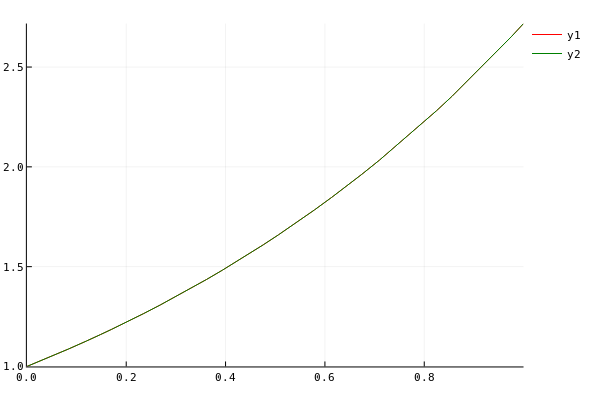
\includegraphics[width=0.8\linewidth]{wykres5a.png}
	\caption{Wykres funkcji $e^{x}$ na przedziale $[0,1]$  dla $n = 5,10,15$}
\end{figure}
	\begin{figure}[H]
	\centering
	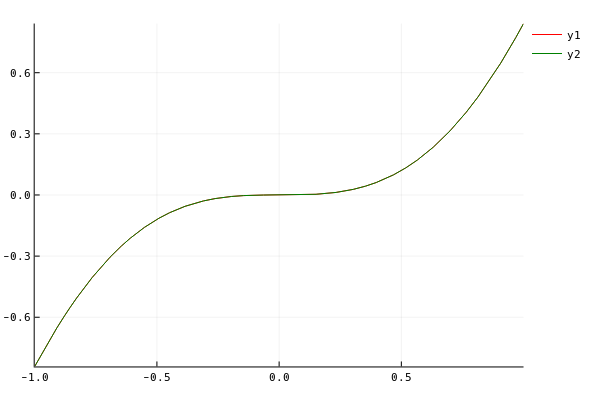
\includegraphics[width=0.8\linewidth]{wykres5b.png}
	\caption{Wykres funkcji $x^2 sin(x)$ na przedziale $[-1,1]$  dla $n = 5,10,15$}
\end{figure}
\subsection{Wnioski:}
Dla zadanych funkcji oraz przedziałów, funkcja $rysujNnfx()$ interpoluje zadane funkcje z bardzo dużą dokładnością. Odchylenia na wykresie są niezauważalne. Ponadto wykres wygląda tak samo dla każdej ilości węzłów zadanej w poleceniu.

\newpage
\section{Zadanie 6}
\subsection{Opis problemu}
Przetestować funkcję $rysujNnfx(f,a,b,n)$ na następujących przykładach (zjawisko rozbieżności):\\
\begin{enumerate}
	\item $|x|$ , $[-1,1]$, $n=5,10,15$,
	\item $\frac{1}{1+x^2}$, $[-5,5]$, $n=5,10,15$
\end{enumerate}
\subsection{Rozwiązanie}
Odpowiednie wywołanie metody $rysujNnfx()$ z zadanymi parametrami.
\subsection{Wyniki}
\begin{figure}[H]
\centering
\begin{minipage}{0.49\textwidth}
	
	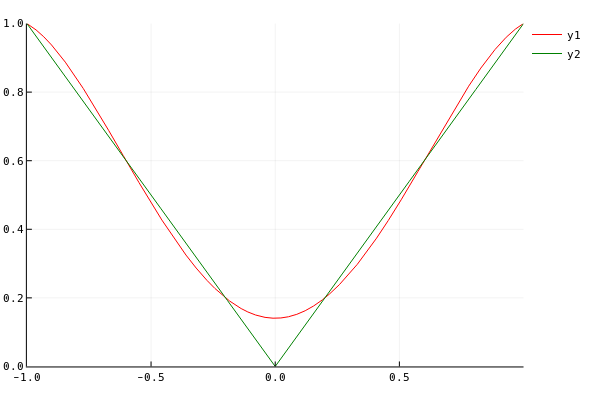
\includegraphics[width=0.8\linewidth]{wykres6a5.png}
	\caption{Wykres funkcji $|x|$ \newline na przedziale $[-1,1]$  dla $n = 5$}
	
\end{minipage}
\begin{minipage}{0.49\textwidth}
	
	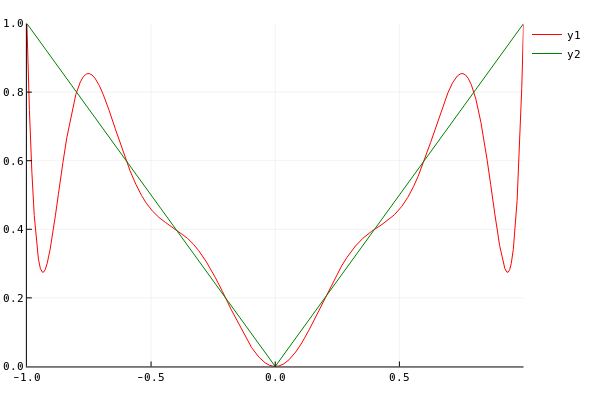
\includegraphics[width=0.8\linewidth]{wykres6a10.png}
	\caption{Wykres funkcji $|x|$ \newline na przedziale $[-1,1]$  dla $n =10$}
\end{minipage}
\end{figure}
\begin{figure}[H]
	\centering
	\begin{minipage}{0.49\textwidth}
		
		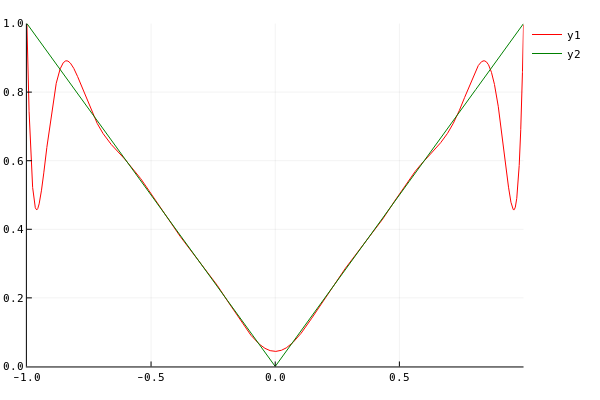
\includegraphics[width=0.8\linewidth]{wykres6a15.png}
		\caption{Wykres funkcji $|x|$ \newline na przedziale $[-1,1]$  dla $n =15$}
		
	\end{minipage}
	\begin{minipage}{0.49\textwidth}
		
		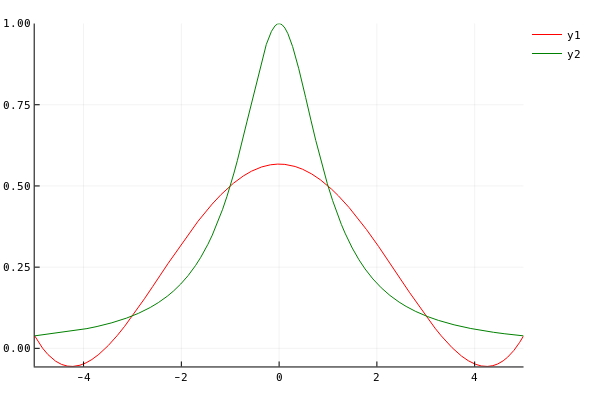
\includegraphics[width=0.8\linewidth]{wykres6b5.png}
		\caption{Wykres funkcji $\frac{1}{1+x^2}$\newline na przedziale $[-5,5]$  dla $n = 5$}
	\end{minipage}
\end{figure}
\begin{figure}[H]
	\centering
	\begin{minipage}{0.49\textwidth}
		
		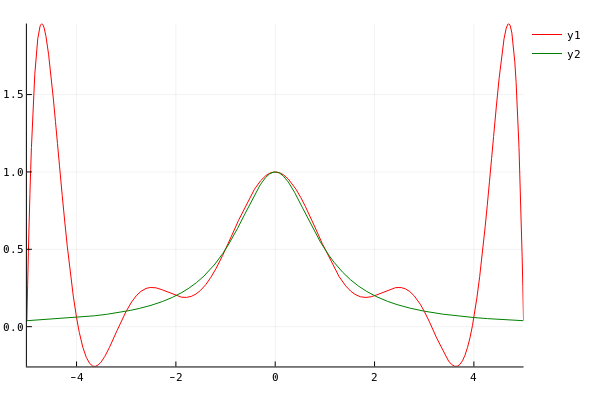
\includegraphics[width=0.8\linewidth]{wykres6b10.png}
		\caption{Wykres funkcji $\frac{1}{1+x^2}$ \newline na przedziale $[-5,5]$  dla $n = 10$}
		
	\end{minipage}
	\begin{minipage}{0.49\textwidth}
		
		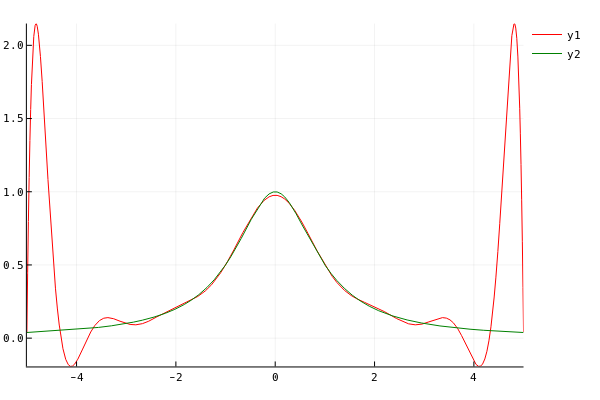
\includegraphics[width=0.8\linewidth]{wykres6b15.png}
		\caption{Wykres funkcji $ \frac{1}{1+x^2}$ \newline na przedziale $[-5,5]$  dla $n = 15$}
	\end{minipage}
\end{figure}
\subsection{Wnioski}
Możemy tutaj łatwo zauważyć, że początkowo wraz ze wzrostem liczby węzłów przybliżenie poprawia się w środkowej części przedziału, jednak tracąc swoją wartość na końcach. Jest to tak zwany efekt Rungego. Jest to typowe zachowanie dla interpolacji za pomocą wielomianów wysokich stopni, przy stałych odległościach węzłów. Dodatkowo funkcja $|x|$ nie jest funkcją gładką co również ma wpływ na interpolację. Aby tego uniknąć można by zastosować węzły coraz gęściej upakowane na krańcach przedziału. Np. dla interpolacji n-punktowej węzłami powinny być miejsca zerowe wielomianu Czybyszewa $n$-tego stopnia.

\end{document}